\section{Distributed Model Checking} \label{sec::DMC}
In addition to benefiting from the isolation of actors for reducing the size of state space, this property can be used for more efficient analysis of a large state space. A major limiting factor in applying model checking for the analysis of real-world systems is the amount of memory space and the time required to store and explore state space. Distributed model checking is a technique for analyzing the state space
%in which it 
where the state space is partitioned into slices, and each slice is assigned to a computational node to be analyzed. Efficiency of this technique depends on the %number of required
amount of communications among the computational nodes which is affected by the distribution policy of states among the nodes \cite{DBLP:journals/entcs/OrzanPE05}. 

To reduce the 
%number of 
amount of required communication among the nodes, split transitions have to be avoided; a split transition is a transition between two states where the hosts of the source and destination states are located at different nodes. In \cite{DBLP:journals/eceasst/KhamespanahSMSR15}, we show how
%the actor model can be used to 
for an actor model we can
reduce the number of split transitions. We introduce a new state distribution policy based on the so-called \textit{Call Dependency Graph (CDG)} of actor models. A CDG represents the abstract causality relation among %messages 
the message passing of actors. Our abstraction is inspired from the Clinger's event diagram \cite{clinger} that shows the trace of system events and causality relation among events. It also can be count as an special kind of System Dependence Graph in which its intra-procedure dependency relations are omitted. \cite{DBLP:conf/scam/Graf10}

In a Clinger's diagram, events are arrival of messages to receivers' message queues. A Clinger's event diagram comprises vertices (called \emph{dots}) for each event, and edges (called \emph{arrows}) that represent the activation relation of two events. Clinger's event diagram is typically drawn using parallel vertical swim-lanes for each actor, where the dots are placed for each event respecting their sequential execution order. Figure~\ref{fig::clinger} represents the Clingers' event diagram of a simple actor model, shown in Listing~\ref{src::actor-model}. In contrast, sent messages of actors are events in CDG and events are associated with edges instead of vertices. The other major difference between Clinger's event diagram and CDG is that Clinger's event diagram is an infinite graph which shows trace of events in actor programs. However, a CDG is generated for an actor model using static analysis of its source code and can accurately represent the flow of message passing among actors. A CDG shows that by handling a message, which messages \emph{may} or \emph{must} be sent to other actors. The idea of dividing edges to \emph{may} and \emph{must} is inspired from \cite{DBLP:conf/lics/LarsenT88} and as we will show later, it helps in having a more effective state distribution policy. Figure \ref{fig::cdg} illustrates the CDG which corresponds to the actor model of Listing~\ref{src::actor-model}.

\begin{lstlisting}[language=rebeca, caption= A simple actor model (from \cite{DBLP:journals/eceasst/KhamespanahSMSR15}), label=src::actor-model]
reactiveclass AC1 {
   knownrebecs {AC2 ac2;}
   AC1() {
     self.msg1();
   }
   msgsrv msg1() {
     self.msg2();
     ac2.msg3();
   }
   msgsrv msg2() {
     self.msg1();
     ac2.msg4();
   }
}
reactiveclass AC2 {
   knownrebecs{AC1 ac1;}
   statevars{int sv;}
   AC2() {
     sv = 1;
   }
   msgsrv msg3() {
     ac1.msg1();
   }
   msgsrv msg4() {
     if (sv == 1)
       sv = 4;
     else
       sv = 3;
   }
}
main {
    AC1 ac1(ac2):();
    AC2 ac2(ac1):();
}
\end{lstlisting}

\begin{figure}
\centering
%\subfigure[Clinger event diagram of the actor model in Listing \ref{src::actor-model}]{
\begin{subfigure}[b]{0.2\textwidth}
  \centering
  \small{
   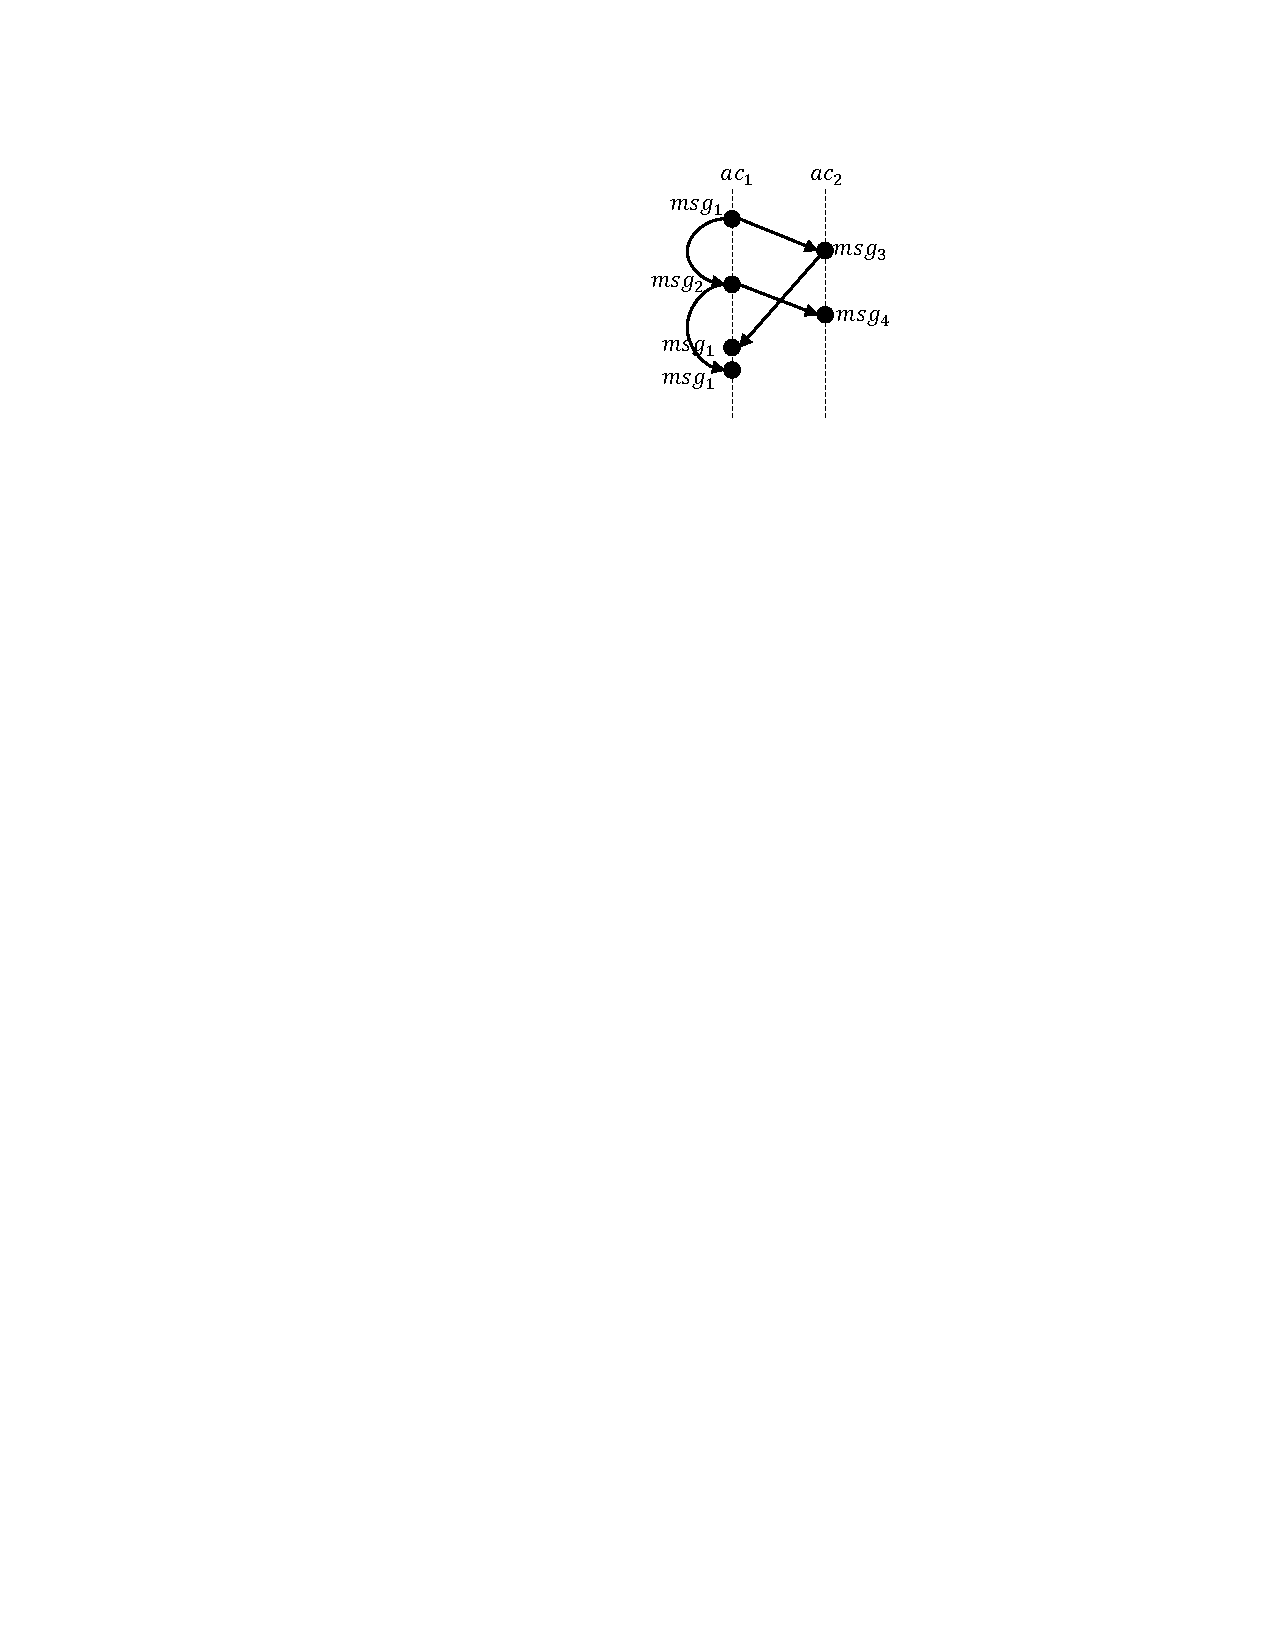
\includegraphics[width=.8\textwidth]{resources/clinger.pdf}
  }
  \caption{Clinger event diagram of the actor model in Listing \ref{src::actor-model}}
  \label{fig::clinger}
%}
\end{subfigure}
\qquad
\begin{subfigure}[b]{0.2\textwidth}
%\subfigure[CDG of the actor model in Listing 1]{

  \centering
  \small{
   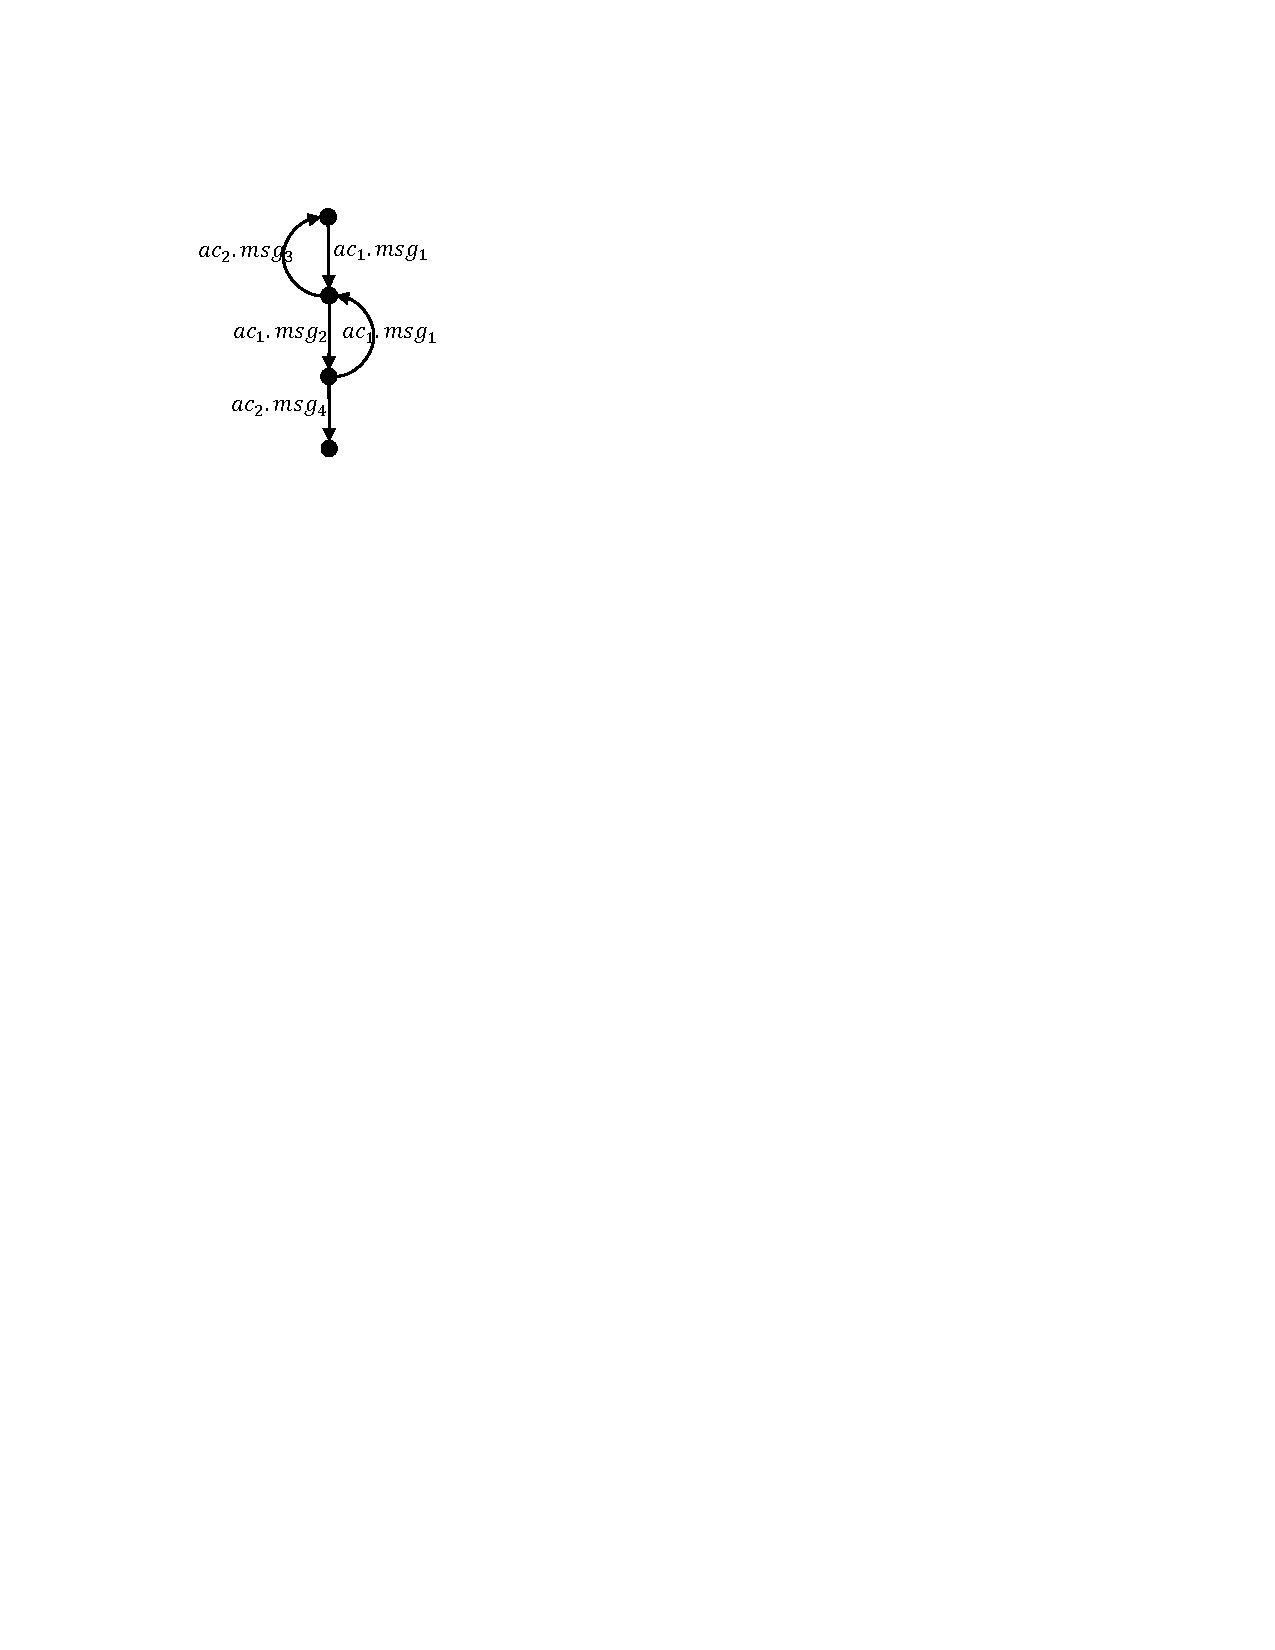
\includegraphics[width=.8\textwidth]{resources/cdg.pdf}
  }
  \caption{CDG of the actor model in Listing \ref{src::actor-model}}
  \label{fig::cdg}
%}
\end{subfigure}
\caption{Clinger event diagram and CDG of the actor model in Listing \ref{src::actor-model} (from \cite{DBLP:journals/eceasst/KhamespanahSMSR15}).}
\label{fig::clinger-cdg}
\end{figure}

The most primitive and widely used distribution policy is the random state distribution \cite{DBLP:journals/entcs/GaravelMS13}. Random state distribution policy distributes states among nodes based on their hash values. Random distribution policy guarantees load balancing. However, it is not an effective technique as it scatters cycles in state spaces over different nodes. Note that detecting cycles of state spaces is crucial for model checking against LTL-like properties; so, splitting them among nodes (i.e., reducing locality of cycles) dramatically increases the time consumption of model checking. % time consumption. %In \cite{DBLP:journals/entcs/OrzanPE05}, another state space distribution policy is suggested to improve the locality of cycles. This policy is based on the static analysis of an abstracted model and detects \emph{may} or \emph{must} transition relations among states \cite{DBLP:conf/lics/LarsenT88}. Based on this analysis, if two states have a \emph{must} relation, they should be stored in a same node. We use a similar idea in our state distribution policy using CDG by partitioning causality relations of CDGs to \emph{may} and \emph{must} relations. 
%In \cite{DBLP:journals/eceasst/KhamespanahSMSR15} we proved that each cycle in the state space of an actor model 
%is 
%can be mapped to a sub-cycle \Marjan{Why sub-cycle and not cycle?} in the %corresponding CDG of that model. 
%
In \cite{DBLP:journals/eceasst/KhamespanahSMSR15} we proved that there is a relation between cycles in state spaces of actor models 
and cycles in their corresponding CDGs.
%So, associating each cycle of a CDG with a computational node of distributed model checkers eliminates cycles which are scattered among different nodes. 
So, we devise a distribution policy that is based on
associating each cycle of a CDG with a computational node of our distributed model checker. When assigning the states of the state space to different nodes, we assign the state to the node which is associated to the corresponding CDG. This way, we reduce the number of cycles which are scattered among different nodes.
%
%\fixme{fix the following sentence - we need to explain more perhaps - I'll try to do that}
In the case that there is a state in CDG which is shared among more than one cycle, the cycle that contains an edge which is associated with a \emph{must} label determines the host of the state. 
%
%\fixme{fix the following sentence- I'll try to do that}
%In other cases, one of the possible cycles is randomly selected and the new state is distributed to its host. 
When none of the cycles include a \emph{must} label then one of the cycles is randomly selected and the new state is distributed to its host. 
%
We have implemented the CDG-based distribution policy in the distributed model checking tool of Rebeca, and the result of using CDG-based distribution policy is shown in Table~\ref{ranomCDGMCTable-splitedge} for three different examples. Experimental evidence supports that this new policy improves cycles locality, and decreases the model checking time and memory consumptions. % in practice.

%So, we detect the \emph{must} relations among the states of an actor model considering the cycles of its corresponding CDG and putting them in the same node. 

\begin{table*}
 {\scriptsize
 \begin{center}
          \begin{tabular}{|l|l|c|c|c|c|}
        \hline
        \multirow{2}*{Problem}& \multirow{2}*{Size}&\multirow{2}*{\#Transitions}& \multicolumn{3}{c|}{\#Split Transitions} \\
        & & & Random & CDG & improvement\\
        \hline
        \multirow{4}*{{Asynch. Resource Manager}}
        &\bf{4 clients} & 7,76K    & 5,83K      & 4516 & 23\%\\
        &\bf{5 clients} & 83,19K   & 66,52K     & 50,46K & 25\%\\
        &\bf{6 clients} & 1,02M    & 850,74K    & 635,14K & 26\%\\
        &\bf{7 clients} & 14,34M   & 12,30M     & 9,01M & 27\%\\
        \hline
        \multirow{3}*{{Dining Philosophers}}
        &\bf{3 phils} & 10,30K  & 6,97K     & 4,81K & 31\%\\
        &\bf{4 phils} & 206,00K & 154,76K   & 75,86K & 51\%\\
        &\bf{5 phils} & 3,78M   & 3,02M     & 1,60M & 47\%\\
        \hline
        \multirow{4}*{{Train Controller}}
        &\bf{5 trains} & 33,30K     & 26,66K    & 18,17K    & 32\%\\
        &\bf{6 trains} & 265,89K    & 221,61K   & 148,32K   & 34\%\\
        &\bf{7 trains} & 2,30M      & 1,97M     & 1,30M     & 35\%\\
        &\bf{8 trains} & 21,83M     & 19,11M    & 12,40M    & 36\%\\
        \hline
        \end{tabular}
        \end{center}
        }\caption{The number of split edges in the random and the CDG-based distribution policies (from \cite{DBLP:journals/eceasst/KhamespanahSMSR15}).}\label{ranomCDGMCTable-splitedge}
\end{table*}

\Marjan{For using similar techniques in distribution of states to nodes, we can think of System Dependence Graphs (SDG) that is presented as an standard formalism to model structures and dependencies in programs \cite{DBLP:conf/scam/Graf10}. SDGs are the basis for multiple applications in program analysis, such as slicing and testing. Similar to CDGs for actor-based models, SDGs can be used in showing causality relations in models, but for a wider range of textual imperative modeling languages including the model checking languages of Promela \cite{Holzmann:2011:SMC:2029108} and NuSMV \cite{Cimatti:1999:NNS:647768.733923}.
However, as all the dependencies between the statements of models are shown in SDGs, there are many cycles in SDGs which are not related to cycles in the state space. 
So, using SDGs for state distribution policy to localize cycles  most likely will not be practically effective.
The reason that there is a relation among the cycles in the CDG and the state space of an actor model is inherent in the model of computation of actors and their isolation.
Our technique is not limited to Rebeca and applicable to other distributed systems where the unit of concurrency can be modeled as isolated autonomous reactive objects and message passing is the only means of communication. }
%

\Ehsan{--} Comparing to CDG, System Dependence Graphs (SDG) have been became a standard formalism to model structures and dependencies in programs \cite{DBLP:conf/scam/Graf10}. They are the basis for multiple applications in program analysis, such as slicing and testing. The same as CDGs of actor-based models, SDGs can be used in showing causality relations in models, but for a wider range of textual imperative modeling languages including Promela and NuSMV. However, as all the dependencies between the statements of models are shown in SDGs, there are many cycles in SDGs which practically are not related to cycles in state spaces. So, using SDGs for state distribution policy to localize cycles is not practically effective. In contrast, actors in Rebeca are isolated, they don't have shared variables, and serve their messages non-preemptively. So, there is no implicit causality relation among events of Rebeca actors and CDGs structures are very close to the structure of state spaces. 
\Marjan{See my paragraph above this one, with what you are saying these things cannot be said any more. YOu are saying SDGs are too much, then nothing being implicit is no more a bonus - maybe over approximation is a bonus ... but SDGs are over approximating too I guess, so I removed all of these and wrote a vague sentence: "The reason that there is a relation among the cycles in the CDG and the state space of an actor model is inherent in the model of computation of actors and their isolation."
which I don't like ... but there is no time to say anything more precise unless you really know how to say that.
}
In fact, the CDGs give us an over-approximation of the causality relations among the events, but that serves our purpose well enough. Our technique is not limited to Rebeca and applicable to other distributed systems where the unit of concurrency can be modeled as isolated autonomous reactive objects and message passing is the only means of communication. 

\begin{comment} 
The efficiency of this distribution policy is directly related to the accuracy of CDG.
%Clinger's event diagrams can be seen as the detailed representations of CDG.
%\Marjan{it may be more clear if you change the sentence and say: CDG is an abstract representation of Clinger's event diagram, but still it is not clear enough, what is abstracted in CDG? It seems that the place of nodes and edges are changed ... please make it more clear.}
As actors are isolated, the only causality relation among events is expressed by sending a message. So, the causality relation of events in a CDG can be extracted from the source codes of actor models using static analysis. 
This way, we over-approximate the causality relations in CDGs.
\Marjan{Because of the isolation of actors in Rebeca, there is no implicit causality relation among events, and for building the CDGs we extract  the causality relations by static analysis of the Rebeca models. In fact, the CDGs give us an over-approximation of the causality relations among the events, but that serves our purpose well enough. 
}
%
\fixme{Is it an over-approximation because of conditional statements?
Why is CDG more abstract than Clinger's event diagram?
Is Isolation the reason that CDG has a relation with the cycles in the state space?
Can other build the CDG and use the same argument?}
%
Figure \ref{fig::cdg} illustrates the CDG which corresponds to the Clinger's event diagram of Figure \ref{fig::clinger}.


%We designated 
%\fixme{What do you mean designated?}
%the existence of a relation between the cycles in a CDG and the cycles in its corresponding state space in \cite{DBLP:journals/eceasst/KhamespanahSMSR15}. 
%
%\Fatem{It is not clear that how isolation helps in resolving this issue}. 
%As mentioned before, Rebeca actors are completely isolated and the only way of expressing causality among events is the message passing mechanism, explicitly specified in Rebeca models. 

\end{comment}